\documentclass[a4paper,12pt]{article}
\usepackage[utf8]{inputenc}
\usepackage[T1]{fontenc}
\usepackage[french]{babel}
\usepackage{graphicx}
\usepackage{url}

% ajout des librairie pour l'insertion de code
\usepackage{xcolor}
\usepackage{listings}
\lstset{
	basicstyle=\ttfamily,
	stringstyle=\ttfamily\color{green!50!black},
	keywordstyle=\color{blue}\bfseries,
	commentstyle=\color{red!50!black}\itshape,
	showstringspaces=true,
	tabsize=2, frame=single,
	numbers=left, numberstyle=\tiny,
	firstnumber=1, stepnumber=1, numbersep=5pt
	}

% En-tête et pied de page
\usepackage{fancyhdr}
\pagestyle{fancy}

% Déclaration de l'en-tête
\renewcommand{\headrulewidth}{1pt}
\fancyhead[l]{Cube led}
\fancyhead[c]{Documentation}
\fancyhead[r]{\today}

% Déclaration du pied de page
\renewcommand{\footrulewidth}{1pt}
\fancyfoot[l]{Kevin Amando \& \\ Alan Devaud \& \\ Gregory Mendez}
\fancyfoot[c]{T.IS-E2B}
\fancyfoot[r]{page \thepage}

% Information sur le projet (auteur, titre, date,etc.)
\title{Cube à led}
\author{Kevin Amando \& Alan Devaud \& Gregory Mendez}
\date{\today}

\begin{document}

% Title page
\begin{titlepage}
    \begin{center}
        % Logo and some informations
        {\large CFPT Ecole d'informatique - Technicien ES en informatique}\\[0.5cm]
        {\large Travail de semestre inter-degré 2016-2017}\\[0.5cm]
        %\includegraphics[width=0.6\textwidth]{YGCLogo.png}\\[1cm]
        
        % Title
        \rule{\linewidth}{0.5mm} \\[0.4cm]
        { \huge \bfseries Cube à Led \\ Documentation \\[0.4cm] }
        \rule{\linewidth}{0.5mm} \\[1.5cm]
    
        % Author and supervisor
        \noindent
        \begin{minipage}{0.4\textwidth}
          \begin{flushleft} \large
            \emph{Elèves :}\\
            M. Kevin \textsc{Amado} \\
            M. Alan \textsc{Devaud}\\
            M. Gregory \textsc{Mendez}
          \end{flushleft}
        \end{minipage}%
        \begin{minipage}{0.4\textwidth}
          \begin{flushright} \large
            \emph{Enseignants :} \\
            M.~Denis \textsc{Carbone}\\
            M.~Nicolas \textsc{Wanner}
          \end{flushright}
        \end{minipage}
        
        \vfill

        % Bottom of the page
        {\large Version 1.0 du\\ \today}
    \end{center}
\end{titlepage}

\newpage

%Résumé
\section{Résumé}
\newpage

% Table of contents
\tableofcontents
\newpage

% Introduction
\section{Introduction}
Notre projet consiste à améliorer le projet Cube de M. \textsc{Aubert} Jonathan dans le câdre de l'atelier Technicien, qui regroupe les deuxièmes année avec les premières. Nous sommes trois à travailler ensemble. L'objectif est de reprendre le travail réaliser en ajoutant une vue 3D. Notre application doit pouvoir gérer la couleur des Leds. La gestion d'animation est aussi demandée.
\newpage

% Cahier des charges
\section{Cahier des charges}
\textbf{\large{But :}}
\begin{description}
	\item Reprendre le projet CubeLed et l'améliorer.\\
\end{description}

\textbf{\large{Points demandés :}}
\begin{itemize}
	\item[*] Interface 3D
	\item[*] Affichage d'un cube de leds
	\item[*] Intéractions avec le cube
	\item[*] Intéractions avec les leds
	\item[*] Gestion de la couleur
	\item[*] Gestion d'animation
\end{itemize}
\newpage

% Analyse de l'existant
\section{Analyse de l'existant}
\subsection{Représentation du Cube dans l'application}
\noindent Le cube possède huit étages, chaques étage contient huit rangées qui, elles-mêmes contiennent huit Leds. Le Cube à Leds est représenté sous la forme d'un tableau à trois dimensions :
\begin{center}
	\textsc{CubeLED}[x][y][nbImage] = value
\end{center}
\begin{center}
\begin{tabular}{r  l}
	\raggedright{\textbf{CubeLED :}} & Le nom du tableau\\
	\textbf{x :} & Position d'une Led sur l'axe "x"\\
	\textbf{y :} & Position d'une Led sur l'axe "y"\\
	\textbf{nbImage :} & Numéro de l'image (animation)\\
	\textbf{value :} & Valeur stockée\\
\end{tabular}
\end{center}

\vspace{1.5cm} 

\textbf{\large{Explication de la valeur stockée dans \emph{"value"} :}}

\noindent Ce sont les deux premiers paramètres qui sont utiles pour représenter la position d'une Led allumée, c'est donc grâce à la valeur stockée que nous indiquerons au microcontrôleur quelle Led il va devoir allumer. On envoie donc une valeur entre 0 et 255, sous forme binaire. Dans cette chaîne binaire, chaque "1" représente une LED allumée et chaque "0" une LED éteinte.
\vspace{1cm} 

\noindent \textsc{Exemple 1 : CubeLED}[0][0][0] = $128_{10}$ -> $10000000_2$ 
\begin{description}
	\item[->]La dernière Led de la ligne x = 0 / y = 0 est allumée.\\
\end{description}

\noindent \textsc{Exemple 2 : CubeLED}[6][4][0] = $170_{10}$ -> $10101010_2$ 
\begin{description}
	\item[->]Une Led sur deux est allumée sur la ligne x = 6 / y = 4.\\
\end{description}

\noindent \textsc{Exemple 3 : CubeLED}[2][7][0] = $0_{10}$ -> $00000000_2$ 
\begin{description}
	\item[->]Aucunes Leds sont allumées sur la ligne x = 2 / y = 7.\\
\end{description}

\noindent \textsc{Exemple 4 : CubeLED}[8][1][0] = $255_{10}$ -> $11111111_2$ 
\begin{description}
	\item[->]Toutes les Leds sont allumées sur la ligne x = 8 / y = 1.\\
\end{description}


\newpage

\noindent Ce format est utilisé pour simplifier la communication avec le microcontrôleur et la création de fichiers ".cube". Il est aussi important de prendre conscience de l’orientation du Cube en utilisant ce format.

\vspace{0.5cm}

\noindent Voici donc ci-dessous, un schéma représentant le tableau CubeLED. La face droite est l’équivalent des deux premiers index de notre tableau (\emph{CubeLED[x][y]}) et les valeurs affichées sur cette dernière sont les éléments stockés à ces positions.

\vspace{0.5cm}

\noindent Le microcontrôleur analyse la valeur binaire convertie (voir axe Z) et allume une LED à chaque fois qu’elle rencontre un "1".

\vspace{0.5cm}

\noindent Note : Le tableau complet contient des animations, ce schéma représente une seule image qui pourrait être présente dans le tableau.

\begin{center}
	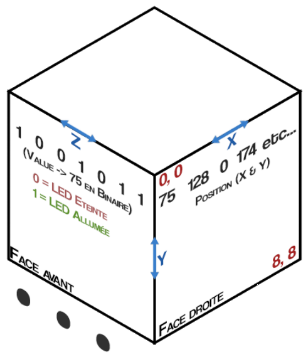
\includegraphics[width=8cm]{./img/schemaCube.png}\\
	\textsc{Figure 1} - Représentation 3D du tableau \emph{CubeLED}
\end{center}

\newpage

\subsection{Format ".cube"}
\noindent Le fichier cube est construit en trois catégories principales :
\begin{itemize}
	\item[*] En-tête du fichier (ASCII)
	\item[*] Images du CubeLED
	\item[*] Luminosité
\end{itemize}
Chaque partie du fichier est séparée par des séparateurs de début et fin. Pour indiquer le début d’une partie, on utilise "\#", pour marquer la fin d’une partie on utilise "\$" par convention.

\vspace{0.5cm}


\begin{flushleft}
	\noindent Voici un schéma représentant la structure du fichier ".cube" :
	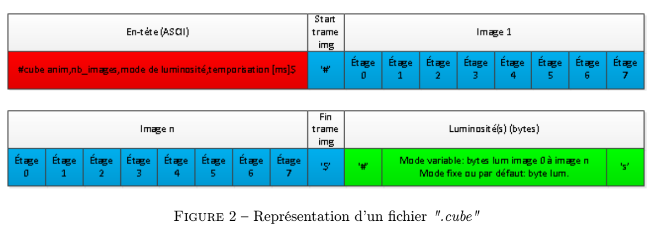
\includegraphics[width=15cm]{./img/structureCube.png}\\
\end{flushleft}
\begin{center}
	\begin{tabular}{|r  l|}
		\hline
		 & \\
		\textbf{\emph{En-tête :}} & Contient les informations relatives à l'animation \\
		\textbf{\emph{Images :}} & Contient les informations sur la position des Leds allumées (par étages) \\
		\textbf{\emph{Luminosité :}} & Si le mode est variable, on indique la luminosité pour chaque image,\\
		 & sinon on indique la luminosité générale du cube. \\
		 & \\
		\hline
	\end{tabular}
\end{center}

\noindent Voici un schéma représentant un étage du cube, un étage contient huit lignes de leds :
\begin{center}
	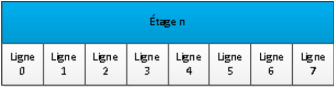
\includegraphics[width=10cm]{./img/structureEtage.png}\\
	\textsc{Figure 1} - Représentation d'un étage du \emph{CubeLED}
\end{center}

\newpage
% Analyse fonctionnelle
\section{Analyse fonctionnelle}
\newpage

% Analyse organique
\section{Analyse organique}
\newpage

% Conclusion
\section{Conclusion}

\newpage

% Pictures table
\newpage
\listoffigures


\end{document}